\RequirePackage[abort, l2tabu, orthodox]{nag}
\documentclass[pageno]{jpaper}

% standard LaTeX packages that do not interfere with hyperref
\usepackage{alltt}
\usepackage{amssymb}
\usepackage{booktabs}
\usepackage{caption}
\usepackage[draft]{fixme}
\usepackage{epstopdf}
\usepackage{flushend}
\usepackage{graphicx}
\usepackage[final]{listings}
\usepackage[sort&compress]{natbib}
\usepackage{tikz}
\usepackage[normalem]{ulem}
\usepackage{xspace}

% font selection
\usepackage{courier}
\usepackage{helvet}
\usepackage{mathptmx}
\usepackage{microtype}
\usepackage[mathscr]{euscript}

% hyperref itself
\usepackage{hyperref}

% standard packages that must be loaded after hyperref
\usepackage{bookmark}
\usepackage{verbatim}

% should be loaded after listings and subfig
\usepackage{cleveref}
\usepackage{multirow}
\usepackage{xfrac}

% custom packages for this paper
\usepackage{xcolor}

%\DeclareCaptionType{copyrightbox}

\renewcommand{\cite}[1]{%
  \PackageError{natbib}{%
    The \string\cite\space{} command is ambiguous; use
    \string\citet\space{} or \string\citep\space{} instead}{}}

\renewcommand{\autoref}[1]{%
  \PackageError{cleveref}{%
    Do not use \string\autoref.  Use \string\cref instead, or use
    \string\crefrange for ranges of referenced items}}

\renewcommand{\hline}[1]{%
  \PackageError{booktabs}{%
    Do not use \string\hline.  Use \string\toprule, \string\midrule,
    or \string\bottomrule\space instead depending on where in the
    table the line appears}}

\newcommand{\email}[1]{\href{mailto:#1@cs.cmu.edu}{#1}}

% cleveref configuration
\crefname{figure}{Figure}{Figures}
\crefname{section}{Section}{Sections}
\crefname{table}{Table}{Tables}

\hyphenation{test-case}

% lst configuration
\lstdefinelanguage{example}{%
  morekeywords={xyz},
}

\lstset{
  basicstyle=\sffamily,
  columns=fullflexible,
  numbersep=5pt,
  numberstyle=\scriptsize,
  showstringspaces=false,
  language=example,
  escapeinside={/*@}{@*/},
  belowcaptionskip=1\baselineskip,
  language=C,
  showstringspaces=false,
  keywordstyle=\bfseries,
  commentstyle=\itshape,
}


\urlstyle{sf}

\pdfpagewidth=8.5in
\pdfpageheight=11in


% Custom commands
\newcommand{\Tool}{\textsc{XYZ}\xspace}

%\sloppy
% start doc
\begin{document}

\title{
  \textsc{\LARGE Midway Report\\
  \Large Automatic Tuning of DBMS using Machine Learning\\
  \large CMU 10-701: Machine Learning (Fall 2014)}
}

\author{Joy Arulraj \hspace{0.1 in} Ram Raghunathan \hspace{0.1 in} \\
{\{\email{jarulraj}, \email{rraghuna}\}}}

\date{}
\maketitle


\begin{abstract}
Modern database systems are highly configurable and must support a
wide variety of workloads. However, \textit{tuning} these systems is
challenging. Configuration assistants like Microsoft's AutoAdmin
\citep{agrawal03} allow administrators to use statistics and
suggestions from the database
system to guide the physical design of the database. However, these methods
still require experienced administrators and prior knowledge about the
workload. We seek to apply machine learning methods to automate database
system tuning with minimal user input and knowledge by matching
workloads to representative benchmarks. In this midway
report, we discuss the our progress on the workload mapping problem.
\end{abstract}

\section{Introduction} \label{sec:intro}

\subsection{Motivation}

DBMS tuning is a niche skill that involves configuring the DBMS suitably for the
underlying hardware as well as guiding the physical design of the database.
Doing these tasks effectively requires a deep knowledge of the SQL workload to
be run on the DBMS, extensive prior experience in DBMS tuning, as well as
significant amounts of time-consuming experimentation with candidate
configurations. This issue is prevalent across several widely used database
management systems. For instance, Robert Hass, a core developer of PostgreSQL, 
stated that \citep{hass12} :

\begin{displayquote}
``On one test, involving 32 concurrent clients, I found that wal\_buffers = 64
MB doubled performance as compared with wal\_buffers = 16 MB; however, on
another system, I found that no setting I tried produced more than a 10 \%
improvement over the auto-tuning formula.'' 
\end{displayquote}

We therefore propose applying machine learning methods to automate the process
of tuning the DBMS for a particular workload on a specific machine.

\subsection{Problem definition}

We address two problems in this project.
First, we try to \textit{map} a given workload comprised of
a set of SQL transactions to a standard database benchmark workload. 
This problem is independent of the underlying DBMS or hardware configuration.
This will allow us to use prior knowledge about the standard 
benchmark gained from previous DBMS deployments. 

We collect features that characterize the SQL workload as well as 
DBMS statistics.
We then use unsupervised techniques like clustering
and supervised techniques like decision-trees 
for mapping the workload.
Performance analysis of the resulting classifier is done via
cross-validation.

Second, we plan to \textit{estimate} the DBMS performance given a 
DBMS configuration, hardware setup and SQL workload. 
This is done with supervised techniques like 
Gaussian process regression.
We use the lasso regression estimator to identify key features 
that influence the throughput and average transactional latency 
of the DBMS.
Performance analysis of the estimator is also done using 
cross-validation.
We describe our progress on solving these problems in this report.

The goals of this project are the following : 
\begin{itemize}
  	\item to create a workload mapper that maps an arbitrary SQL workload to a
well-known standard benchmark
	\item to estimate the performance metrics of a DBMS given a workload and
configuration pair
\end{itemize}

We first describe how we generate the dataset in \cref{sec:data_set}. 
Then, we focus on the feature extraction problem in \cref{sec:features}.
We describe our experimental setup and dataset information in
\cref{sec:eval}. The evaluation results obtained for the classification
problem and the estimation problem are shown in \cref{sec:classfication}
and \cref{sec:estimation} respectively. Finally, we present the 
conclusions of this project in \cref{sec:conclusion}.
\section{Data Set} \label{sec:data_set}

The dataset required for this project would ideally comprise of a 
collection of real world SQL workloads, DBMS configurations and performance
metrics. Collecting and curating such a dataset is itself an interesting
problem.
However, in this project, we first want to experiment with a smaller dataset
to better understand the features relevant for our learning problem.
Therefore, we chose to generate the dataset using
OLTP-Bench~\citep{oltpbench14}, an extensible DBMS benchmarking framework.
We use the SQL workloads of standard benchmarks already available
in OLTPBench. 

We generate more synthetic variants of these workloads for training and
testing purposes. As we mentioned earlier, while this synthetic data will not be
representative of real-world workloads, we feel it is a good starting point for
evaluating viability of the approach outlined above.
We extract several features from the workload such as types of database queries,
distribution of query types, and table access patterns using 
a workload analyzer. We hook this analyzer into Postgres~\citep{postgres91} to collect 
features from the DBMS.

The key reasons for why we use OLTP-Bench framework to generate the dataset 
are the following:

\begin{itemize}
  \item It supports several relational DBMSs through the JDBC interface
  including Postgres, MySQL, and Oracle.
  \item It allows us to control the workload mixture in a benchmark. For
  instance, we can adjust the percent of read and update transactions in 
  the YCSB~\citep{ycsb} benchmark to generate different variants of the workload.
  \item It supports user-defined configuration of the rate at which the
  transaction requests are submitted to the DBMS. This allows us to emulate
  different world workloads with varying degrees of concurrency.
  \item It exposes statistics that are complementary to the 
  internal statistics of the DBMS~\citep{postgres14}. We extract features from
  these statistics.
\end{itemize}

We implemented a dataset generator that runs different benchmarks supported
by OLTP-Bench on a Postgres DBMS. After every workload execution, we
collect statistics from the DBMS as well as from the testbed. We alter the
workload mixture in all the benchmarks to generate different variants and
emulate real world workloads. The key characteristics of the benchmarks
that we use for generating the dataset are presented in \cref{tab:benchmarks}.

\begin{table*}[ht!]
  \centering
  \begin{adjustbox}{max width=\textwidth}
  \begin{tabular}{l|lllllllll} \toprule
   Benchmarks & Tables & Columns & Pr. & Indexes &	Fr. & 
   Txn. & \# of & Application  & Attributes  \\
   & & & Keys & & Keys & Types & Joins  & domain & \\
   \midrule
	AuctionMark 	& 16 	& 125  &	16 &	14 &	41 &	10 &	10 &	Online &
	Non-deterministic\\
	& & & & & & & & Auctions &  heavy transactions \\
	Epinions 		& 5 	& 21   & 	2  &	10 &	 0 & 	9  &	3  &	Social  & Joins over
	many-to- \\
	& & & & & & & & Networking & many relationships  \\
	%JPAB 	7 	68 	6 	5 	3 	4 	N/A 	Object-Relational Mapping 	Bursts of random%reads, pointer chasing 
	%ResourceStresser 	4 	23 	4 	0 	0 	6 	2 	Isolated Resource Stresser 	CPU-,disk-, lock-heavy transactions 
	SEATS &	10 &	189 &	9 	& 5 	& 12 	& 6 &	6 &	Online Airline  &
	Secondary indices queries\\
	& & & & & & & & Ticketing & foreign-key joins \\
	TATP &	4 	& 51 &	4 &	5 &	3 &	7 &	1 &	Caller Location  &	Short, read-mostly\\
	& & & & & & & & App & non-conflicting\\
	& & & & & & & & &  transactions\\
	TPC-C &	9 &	92 &	8 &	3 &	24 &	5 &	2 &	Order Processing & Write-heavy
	transactions\\
	Twitter &	5 &	18 &	5 &	4 &	0 &	5 &	0 &	Social Networking & Client-side joins \\
	& & & & & & & & & on	graph data \\
	Wikipedia &	12 &	122 &	12 &	40 &	0 &	5 &	2 &	Online &	Complex	transactions \\ 
	& & & & & & & & Encyclopedia & large data, skew  \\
	YCSB &	1 &	11 &	1 &	0 &	0 &	6 &	0 &	NoSQL store &	Key-value queries \\
   \bottomrule
   \end{tabular}
   \end{adjustbox} 
\caption{Key characteristics of the benchmarks used in our evaluation. ``Pr. key''
denotes primary key and ``Fr. key'' denotes foreign key.}
\label{tab:benchmarks}
\end{table*}



\section{Feature Extraction} \label{sec:features}

We collect 3 types of features from both the DBMS as well as the benchmarking
framework.

\subsection{Features from OLTP-Bench }

  After executing the benchmark, we obtain statistics about the latency and
  throughput delivered by the DBMS.
  This includes both temporal performance metrics as well as aggregate metrics. 
  We then record the size of the workload also known as the
  \textit{scalefactor}.
  The \textit{isolation level} of the DBMS correlates strongly with performance
  metrics Stricter isolation levels like ``serializable level'' correlate with lower
  performance because the DBMS needs to maintain the constraints regarding
  the visibility of effects of concurrent transactions. 
  
  We also record the type
  of DBMS used. Although currently we focus only on Postgres, 
  we anticipate this tool to be useful for other DBMSs as well.   
  We also record the expected label i.e. the benchmark name. This is used for
  evaluating the accuracy of our classification algorithms.  
  
\subsection{Static parameters from Postgres}

  Static parameters are features that do not vary over every execution. This
  primarily includes the configuration parameters of the DBMS and the hardware
  setup.
  For example, these are some of the static parameters that we use as features:\\
   
  \begin{itemize}
    \item {Size of shared memory buffers: This impacts the performance of
    memory-intensive queries significantly.}
    \item {Background writer delay: The background writer issues writes of
    dirty shared buffers to disk. This increases the net overall I/O load but
    allows server processes to avoid waiting for writes to finish.}
    \item {Vacumm cost delay: The vacumm process performs garbage 
    collection. Very short delays can impact the DBMS performance.}
    \item {WAL level: The type of write-ahead logging performed - minimal,
    archive, or hot standby - affects the logging overhead.}
    \item {\textit{fsync}: Durability requirements of data.}
    \item {Sequential page cost: Used in the cost model of the DBMS' planner.}
	\item {Hardware features: CPU cache sizes, DRAM size, disk size, cache latency,
	DRAM latency and disk latency.}
  \end{itemize}
  
  Overall, these metrics significantly impact the performance of the DBMS. A
  non-expert user might not be able to configure these parameters to obtain
  good performance. Our tuning tool can help such users by automatically
  identifying a good DBMS configuration for a given workload.  
  
\subsection{Dynamic parameters from Postgres}
  
  We also collect dynamic parameters from the DBMS during feature extraction.
  To do this, we implemented a Postgres driver that queries the DBMS's internal
  catalog tables like pg\_stat\_database, pg\_statio\_user\_indexes,
  pg\_stat\_activity and pg\_stat\_user\_table
  to obtain useful workload parameters. For instance, these are some of the
  dynamic parameters that we use as features :\\
  
  \begin{itemize}    
    \item {Number of transactions in this database that have been committed or
    rolled back.}
    \item {Number of disk blocks read in this database.}
    \item {Number of times disk blocks were found already in the DBMS's buffer
    cache.}
    \item {Number of rows returned, fetched, inserted, updated or deleted by
    queries in this database.}
    \item {Number of index and cache blocks hit.}
    \item {Status of different storage backends of the DBMS.}
    \item {Size of the tables and indexes in the DBMS.}
    \item {Number of sequential scans and index scans performed by the
    workload.}
  \end{itemize}
  
  	We normalize the relevant metrics by the number of transactions executed.
  	Before the start of an execution, we reset all the statistics using our
  	DBMS driver. Overall, this gives us a nice set of features about the
  	workload. 

After collecting all these features, we transform them to a metric space and
normalize them to generate a feature matrix and a label matrix. This is 
used by the classification algorithms that we describe in the next section.

\section{Evaluation} \label{sec:eval}

To evaluate our algorithms, we decided to use the ``scikit-learn''
\citep{scikit-learn} package for Python. In exploring the best way to
map workloads onto benchmarks, we evaluated both clustering algorithms
as well as SVM. The rest of this section discusses the results we
observed with each method.

\begin{figure*}[h]
    \centering
    \begin{tabular}{c c c c}
      \toprule
      Algorithm                     & Homogeneity & Completeness & V-Measure \\
      \midrule
      K-Means                       & 1.000       & 1.000        & 1.000     \\
      Affinity-Propagation          & 0.824       & 1.000        & 0.904     \\
      Mean-Shift                    & 1.000       & 0.795        & 0.886     \\
      Ward Agglomerative Clustering & 1.000       & 1.000        & 1.000     \\
      DBSCAN                        & 0.000       & 1.000        & 0.000     \\
      \bottomrule
    \end{tabular}

    \caption{Clustering Algorithm Performance Metrics}
    \label{fig:clustering-metrics}
\end{figure*}

Clustering was our first approach as an unsupervised algorithm seemed
to best fit the data at hand. As such, we tried the following methods,
all of which are inbuilt in scikit-learn:

\begin{itemize}
\item K-Mean
\item Affinity Propagation
\item Mean-Shift
\item Ward Agglomerative Clustering
\item DBSCAN
\end{itemize}

The clusters found by each algorithm can be seen in
\ref{fig:clusters}. We also calculated common clustering metrics such
as homogeneity, completeness, and V-measure. These results can be
found in \ref{fig:clustering-metrics}. From the results, we notice
immediately that DBSCAN does not work well with our data. Indeed, it
does not find any distinct clusters at all. However, K-Means and Ward
Agglomerative Clustering are very good. We believe that this is
partially because both of these algorithms require number of clusters
as a parameter, which allows them to find our desired number of
clusters. However, this is not a restriction for our problem as we
know the number of benchmarks - and hence the number of clusters -
that we have.

In addition to evaluating clustering algorithms, we also evaluated
Support Vector Machines, a supervised classifier. While real-world
data will not be labeled and hence a supervised classifier cannot be
used, it is useful to see how effective our features are in
discriminating between benchmarks. Using a simple two-fold
cross-validation, we found that a simple SVM with an RBF kernel
achieved 86\% precision but with a very high standard deviation of
28\%. However, this is still a very strong result as it indicates that
our features effectively separate our data into our desired
classes. 
We plan to validate the classifier on more sophisticated heterogeneous 
real-world workloads as part of our stretch goal.

The immediate goal is to build an estimator that allows us to address the
second goal of this project. We already have the infrastructure required
for collecting metrics and features required for solving this problem.
We plan to explore different machine learning algorithms to achieve this
in the next 2 weeks.
 



\section{Classification} \label{sec:classfication}

We approach the problem of mapping a workload to a standard benchmark class
using two techniques. 

\subsection{Clustering}
\label{sec:clustering}

Clustering was our first approach as an unsupervised algorithm seemed to best
fit the data at hand. 
We evaluated the following clustering algorithms in Scikit.\\

\begin{itemize}
\item \textbf{K-Means} :
This algorithm clusters the samples into groups of similar variance by
minimizing the within-cluster sum-of-squares. The number of clusters
needs to be specified. The algorithms scales well to a large number of
samples.

Given a set of $n$ samples X, the algorithm splits them into $K$ disjoint
clusters, wherein each cluster is defined by the mean $\mu_k$ of the samples in
the cluster i.e. the centroids of the cluster.
The algorithm minimizes the within-cluster sum-of-squares criterion:
$$\sum_{i=0}^{n}\min_{\mu_{k} \in C}(\| x_{k} - \mu_{i} \|^2)$$\\

\item \textbf{Affinity Propagation}:
This algorithm creates clusters by passing messages between pairs of samples
till it reaches convergence. The clusters are described using a small number of
exemplars that are most representative of the dataset.
The messages indicate the suitability of one sample to be the exemplar of the
other and this gets updated over time for the entire dataset.

For a pair of samples $i$ and $k$, the evidence that sample $k$ should be the
exemplar for sample $i$ is defined by:
$$r(i,k) \leftarrow s(i,k) - max [a(i,j) + s(i,j) \forall j\neq k ]$$

Here, $s(i, k)$ is a similarity metric and availability $a(i, k)$ is the
accumulated evidence that sample $i$ should choose sample $k$ as its exemplar.
Thus, the exemplars chosen are similar enough to many samples and are
chosen by many samples to be representative of themselves.\\

\item \textbf{Mean-Shift} :
This algorithm tries to identify blobs in a smooth density of samples. 
It works by first identifying candidates for centroids and then filtering them
to eliminate near-duplicates.

For a candidate centroid $x_i$ in iteration $t$, the algorithm updates
the candidate effectively to be the mean of the samples within its neighborhood:

$$x_{i}^{t+1} = x_{i}^{t} + \frac{\sum_{x_{j} \in N(x_i)}K(x_{j} -
x_{i})x_{j}}{\sum_{x_{j} \in N(x_{i})}K(x_{j} - x_{i})} $$

Here, $N(x_i)$ depicts the neighborhood of samples within a given distance
around $x_i$ and the additive term is basically the mean shift vector 
computed for each centroid that points towards a region of the maximum
increase in the density of points.\\

\begin{figure*}[h!]
    \centering
    \fbox{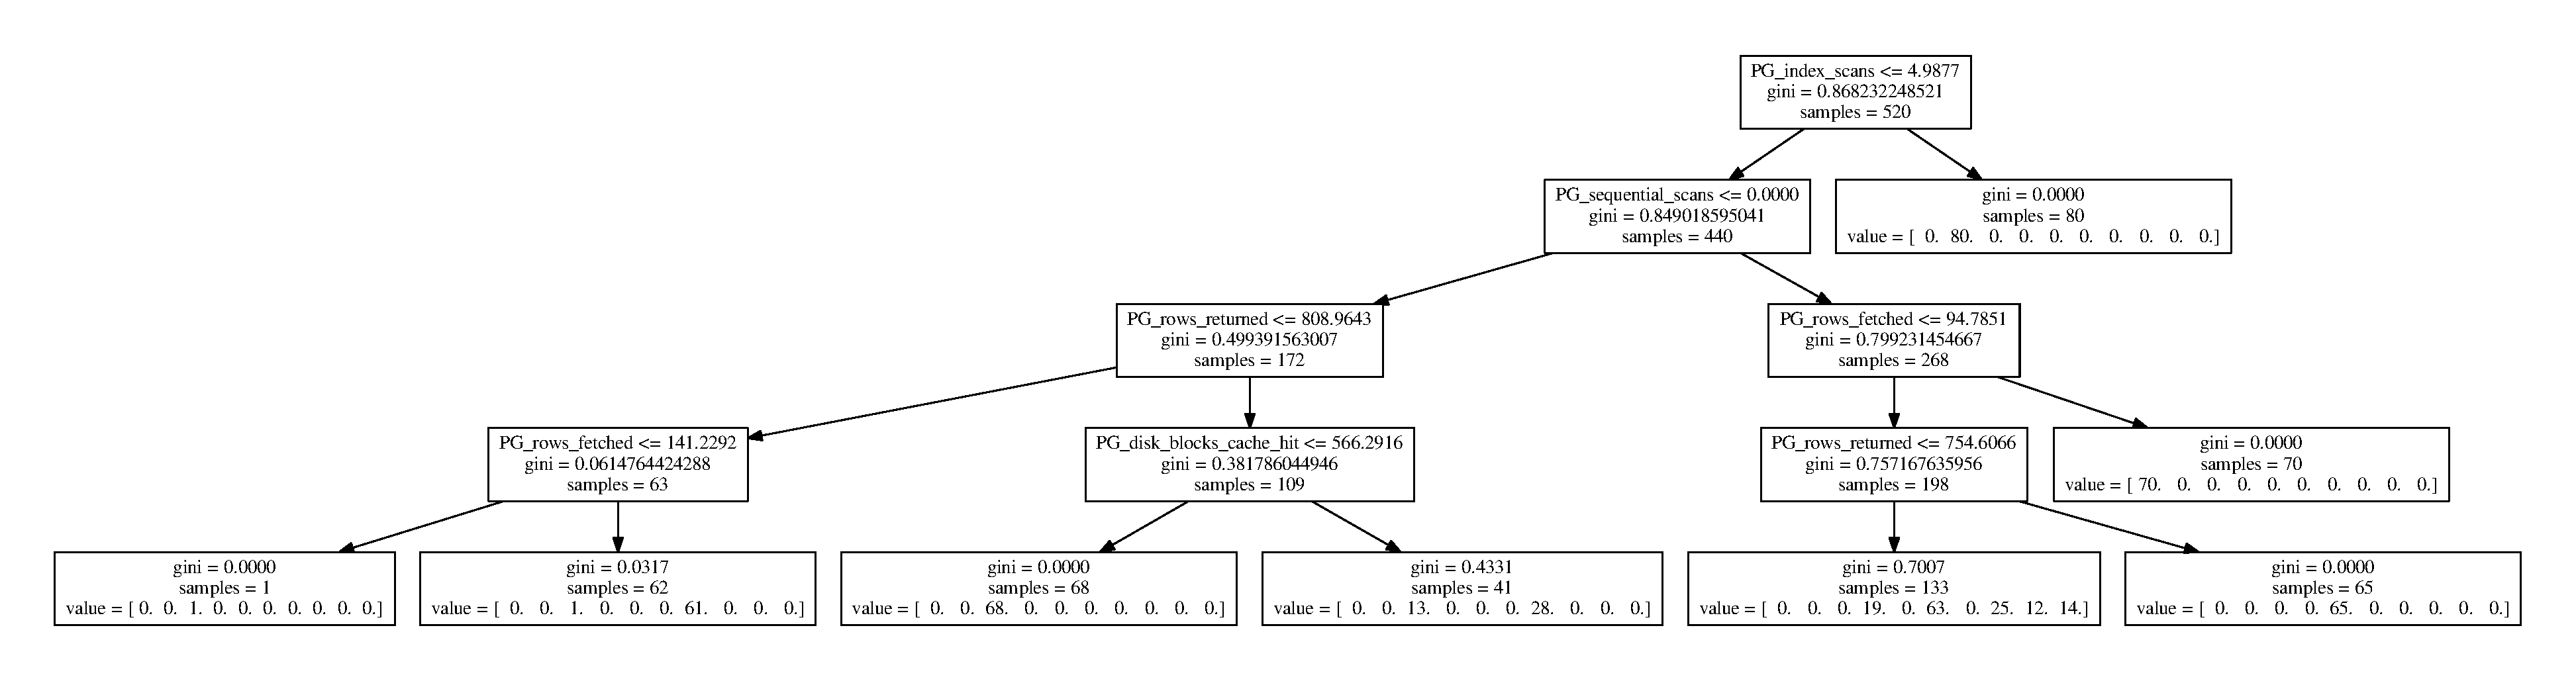
\includegraphics[width=\linewidth]{figure/tree_4.pdf}}
    \caption{Decision tree with max depth set to 4.}
    \label{fig:tree_sample}
\end{figure*}

\begin{figure}[h!]
    \centering
	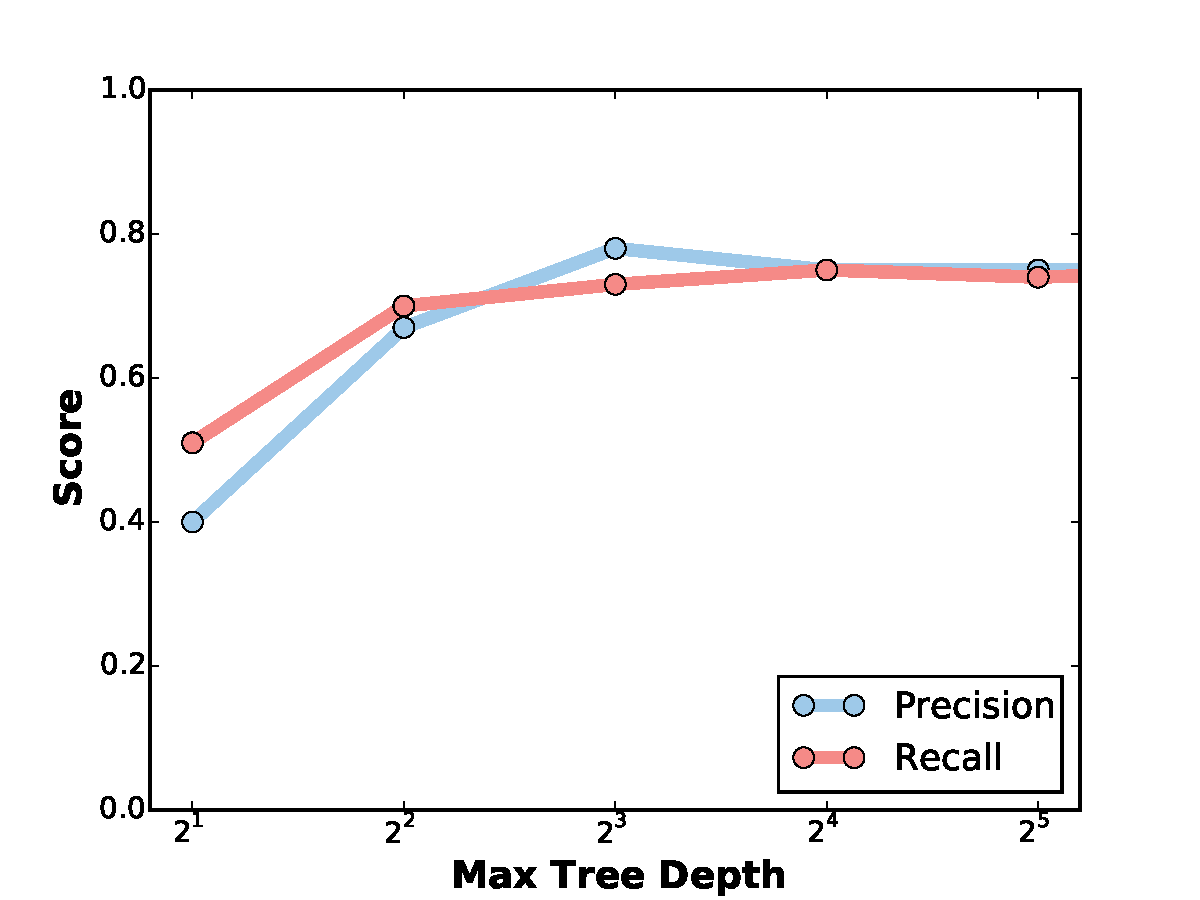
\includegraphics[width=0.7\linewidth]{figure/depth.pdf}
	\caption{Impact of max depth on the accuracy of the decision tree.}
	\label{fig:tree_depth}
\end{figure}

\begin{figure}[h!]
    \centering
	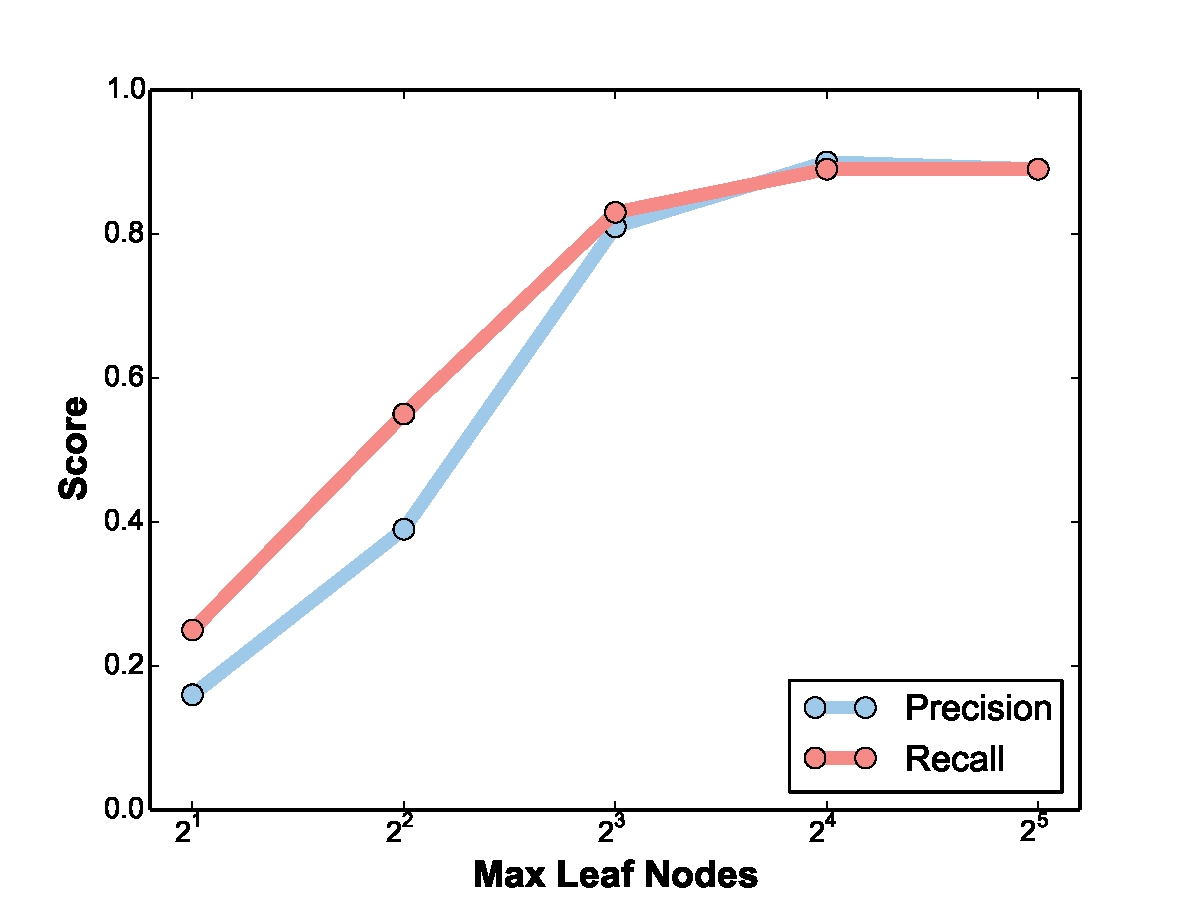
\includegraphics[width=0.7\linewidth]{figure/leaves.pdf}
	\caption{Impact of max leaf nodes on the accuracy of the decision tree.}
	\label{fig:tree_leaves}
\end{figure}

\item \textbf{Agglomerative Clustering} :
This algorithm is a type of hierarchical clustering algorithms that build nested clusters 
by merging or splitting them successively. 
The cluster hierarchy is represented as a tree, wherein the root is the unique
cluster that gathers all the samples and the leaves are the clusters with only
one sample. 
This particular algorithm uses a bottom up approach. Each samples starts in
its own cluster, and over time the clusters are successively merged together
based on a linkage criteria.
We use the \textit{ward} criteria that minimizes the sum of squared differences 
within all clusters that is effectively a variance-minimizing approach.
\end{itemize}

The clusters found by each algorithm in high-dimensional space are shown in
\cref{fig:clusters}.
We computed standard clustering metrics for each algorithm including the
following :\\

\begin{itemize}
  \item \textbf{Homogeneity}:
	Given a ground truth, this metric computes if all the clusters contain only
	data points which are members of a single class.\\

  \item \textbf{Completeness}: 
	Given a ground truth, this metric computes if all the data points that are
	members of a given class are elements of the same cluster.\\

  \item \textbf{V-measure}: 
	This metric is the harmonic mean between homogeneity and completeness
	\citep{v-measure}.

	$$v = 2 * \frac{(homogeneity * completeness)}{(homogeneity + completeness)}$$\\

  \item \textbf{Silhouette coefficient}: 
  This metric is computed using the mean intra-cluster distance
  $a$ and the mean nearest-cluster distance $b$ for each sample.
  It is defined for each sample as $(b-a)/max(a, b)$.\\
\end{itemize}

These results are presented in \cref{fig:clustering-metrics}. We observe that
the clustering algorithms work reasonably well with our dataset
especially the K-Means and Ward Agglomerative Clustering algorithms. 
Both these algorithms require number of clusters as a parameter. 
However, this is not a restriction for our problem as we know the number of
benchmarks - and hence the number of clusters - that we have.
Algorithms like Affinity-Propagation and Mean-Shift give very high and 
very low estimates for the number of clusters in the dataset respectively.
As we required higher classification accuracy and better intuition about
the classifier, we also experimented with SVM classifiers and decision trees. 
We finally decided to use decision trees as they met both our accuracy
and intuition requirements.

\begin{figure*}
\centering
\subfloat[\label{fig:gp_r2_latency}]{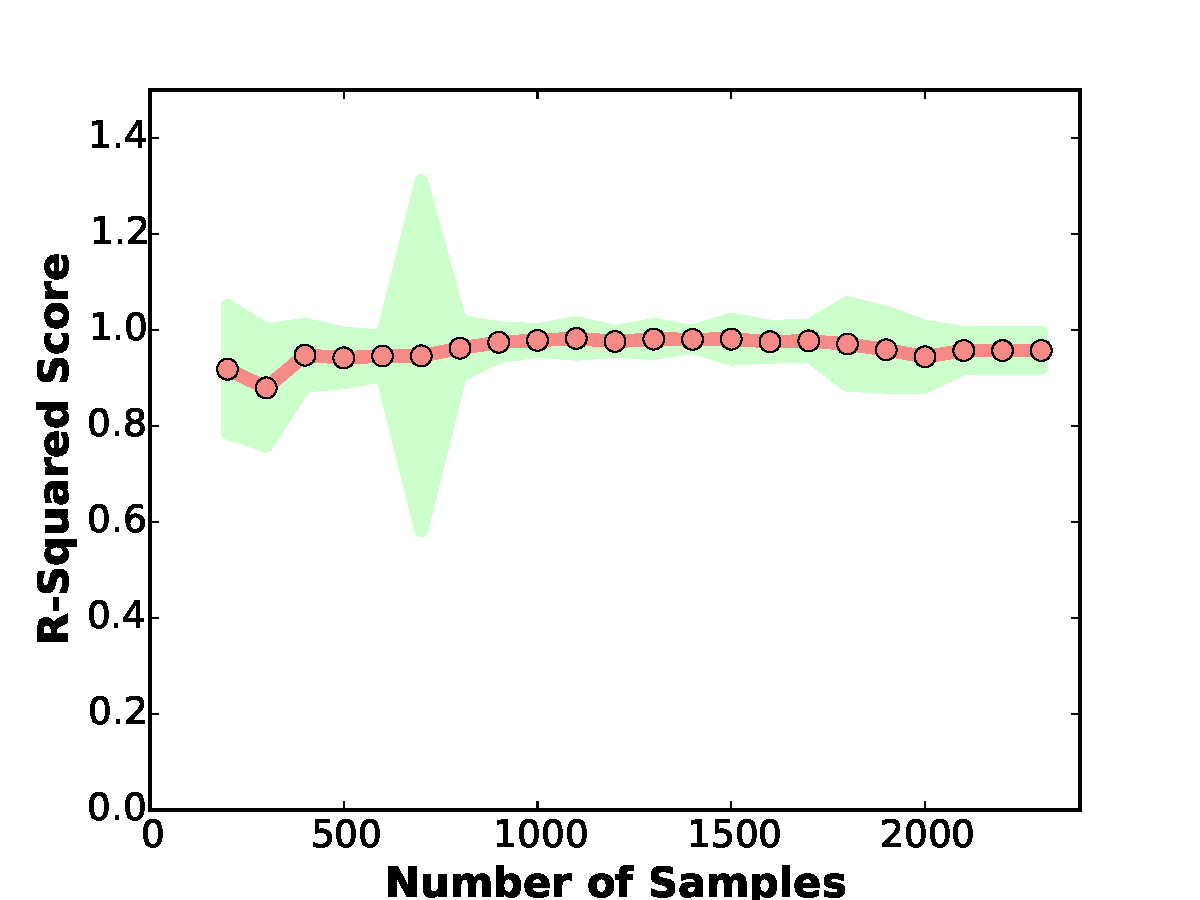
\includegraphics[width=0.4\textwidth]{figure/gp_per_benchmark_r2_scores_latency_mutate.pdf}}
%
\subfloat[\label{fig:gp_r2_throughput}]{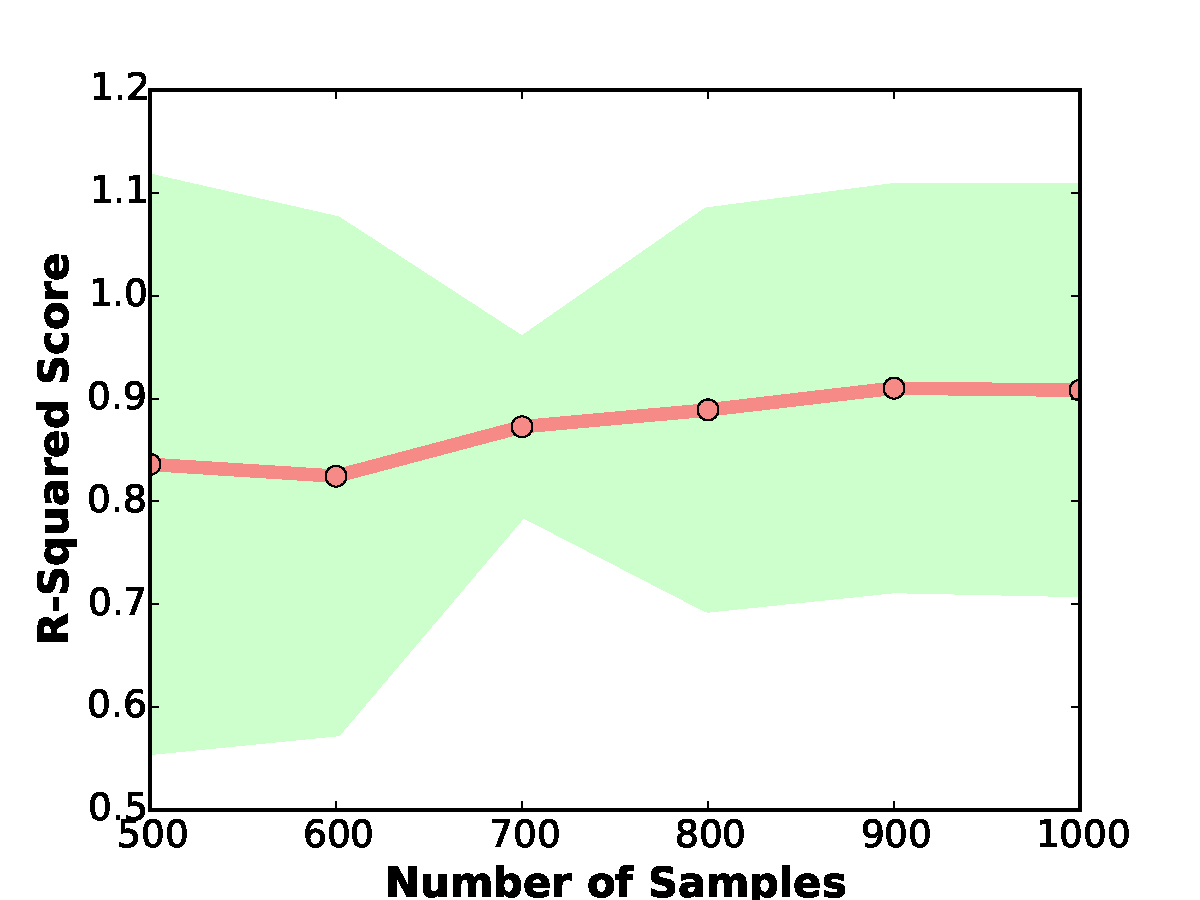
\includegraphics[width=0.4\textwidth]{figure/gp_per_benchmark_r2_scores_throughput_mutate.pdf}}

\caption{Per-benchmark gaussian processes to estimate (a) latency and
  (b) throughput}
\label{fig:gp_r2}
\end{figure*}


\subsection{Decision Trees}
\label{sec:dt}

Decision trees are non-parametric supervised learning algorithms used for
both classification and regression. 
It creates a model for predicting the class of a sample by learning
simple decision rules inferred from the sample features\citep{stats01}.
These trees can be interpreted easily and visualised.
We however need to be careful not to create overly complex trees 
that do not generalise the data well, i.e. we should avoid overfitting. 

Given a set of training samples $x_i \in R^n$, $i=1,...,l$ and the
corresponding label vector $y \in R^l$, the decision tree partitions 
the space recursively so that samples with the same labels are grouped
together.
We denote the data at a node $m$ in the decision tree as $Q$. For
every candidate split $\theta = (j, t_m)$ that consists of a feature $j$ 
and a feature-specific threshold $t_m$, the tree partitions the data into
two subsets $Q_{left}(\theta)$ and $Q_{right}(\theta)$, wherein :
$$Q_{left}(\theta) = {(x, y) | x_j <= t_m}$$ 
$$Q_{right}(\theta) = Q \setminus Q_{left}(\theta)$$

At each node $m$, we compute an impurity measure that we denote by $H$.
$$G(Q,\theta) = \frac{n_{left}}{N_m} H(Q_{left}(\theta)) +
\frac{n_{right}}{N_m} H(Q_{right}(\theta))$$

We search for parameters that minimize $H$:
$$\theta^* = \operatorname{argmin}_\theta G(Q,\theta)$$

We then do the same process recursively for subsets $Q_{left}(\theta^*)$ and
$Q_{right}(\theta^*)$ until we reach the maximum allowable depth or $N_m
< \min_{samples}$ or $N_m = 1$.
For the classification problem where the target is in $[ 0, K-1]$
for node $m$, representing a region $R_m$ with $N_m$ observations, 
the proportion of class $k$ observations in node $m$ is given by :
$$p_{mk} = 1/ N_m \sum_{x_i \in R_m} I(y_i = k)$$
We use the \textit{Gini measure} as the impurity measure:
$$H(X_m) = \sum_k p_{mk} (1 - p_{mk})$$

The implementation uses an optimized version of the CART (Classification and
Regression Trees) algorithm\citep{cart84}.
It basically constructs binary trees using the feature and threshold that
yield the largest information gain at each node.
The features need not be categorical as the algorithm dynamically 
defines a discrete attribute based on numerical variables that 
partitions the continuous attribute value into a discrete set of intervals. 
It does not compute rule sets unlike the C4.5 algorithm\citep{quinlan93}.

A sample decision tree with maximum depth limited to $4$ is shown in
\cref{fig:tree_sample}. We obtain $76\%$ accuracy with this short tree.
The per-class accuracy metrics of the decision tree is shown in 
\cref{tab:dt_stats}.
The precision is the ratio $tp/(tp+fp)$ where $tp$ is the number of true
positives and $fp$ the number of false positives. 
It is intuitively the ability of the classifier not to label 
as positive a sample that is negative.
The recall is the ratio $tp/(tp+fn)$ where $tp$ is the number of true
positives and $fn$ the number of false negatives. It is intuitively the
ability of the classifier to find all the positive samples.
The F1 score is a weighted average of the precision and recall 
and is defined as:
$$F1 = 2 * \frac{(precision * recall)}{(precision + recall)}$$
The support is the number of occurrences of each class in the true label
vector $y\_true$.

These are some interesting observations derived from the decision tree shown in 
\cref{fig:tree_sample}:\\

\begin{itemize}
  \item Wikipedia benchmark performs a lot of index scans.
  \item SEATS benchmark involves fetching several rows per transaction.
  \item Epinions benchmark, on the other hand, involves returning several rows
  per transaction.
  \item Auctionmark benchmark has less locality of reference i.e. the number of
  disk block cache hits is low.
  \item Twitter benchmark also fetches several rows per transaction. However, it
  does not perform any sequential scans.\\
\end{itemize}

\begin{figure*}
\centering
\subfloat[\label{fig:actual_latency_wikipedia}]{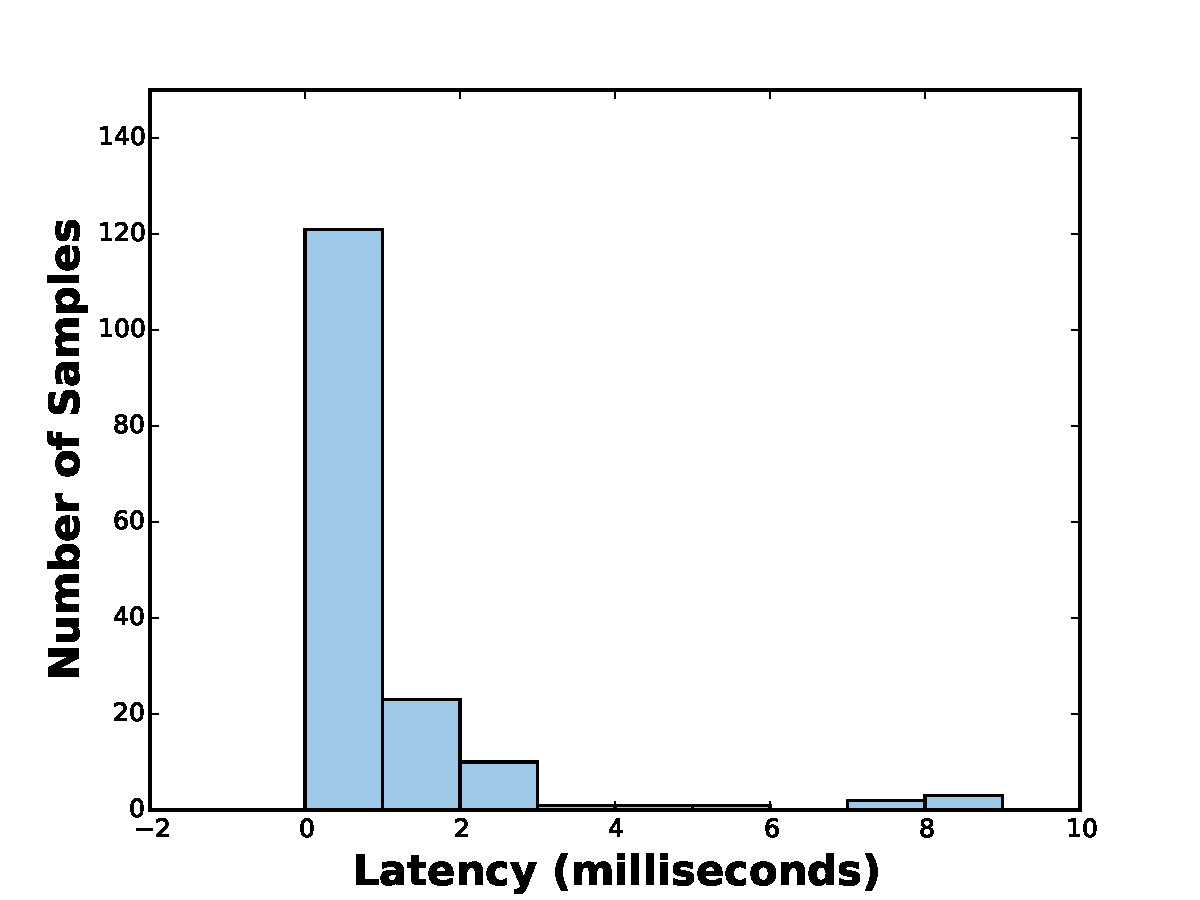
\includegraphics[width=0.4\linewidth]{figure/wikipedia_test_hist_latency_mutate.pdf}}
\subfloat[\label{fig:predicted_latency_wikipedia}]{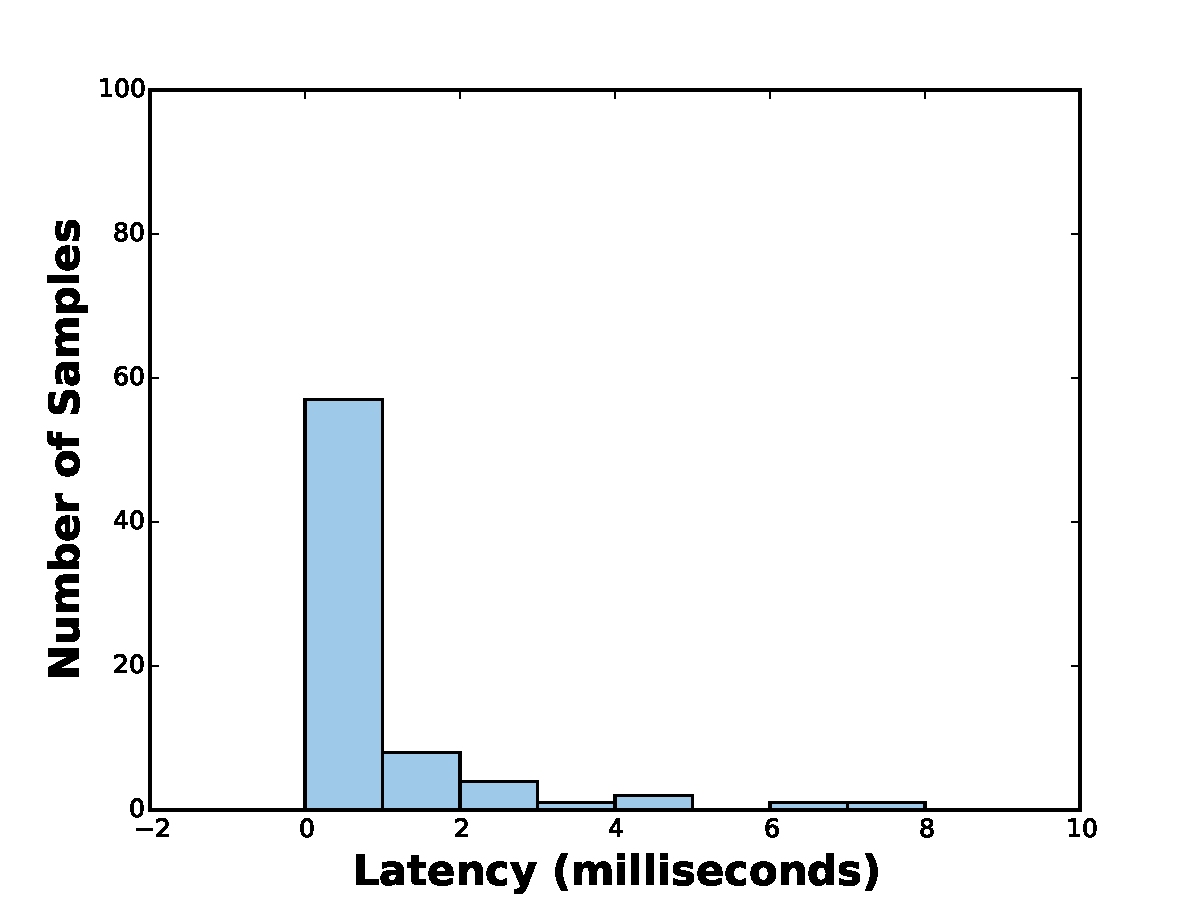
\includegraphics[width=0.4\linewidth]{figure/wikipedia_pred_hist_latency_mutate.pdf}}

\caption{(a) Actual and (b) predicted latency distribution for the
  Wikipedia benchmark}
\label{fig:latency_wikipedia}
\end{figure*}

\begin{figure*}
\centering
\subfloat[\label{fig:actual_throughput_ycsb_balanced}]{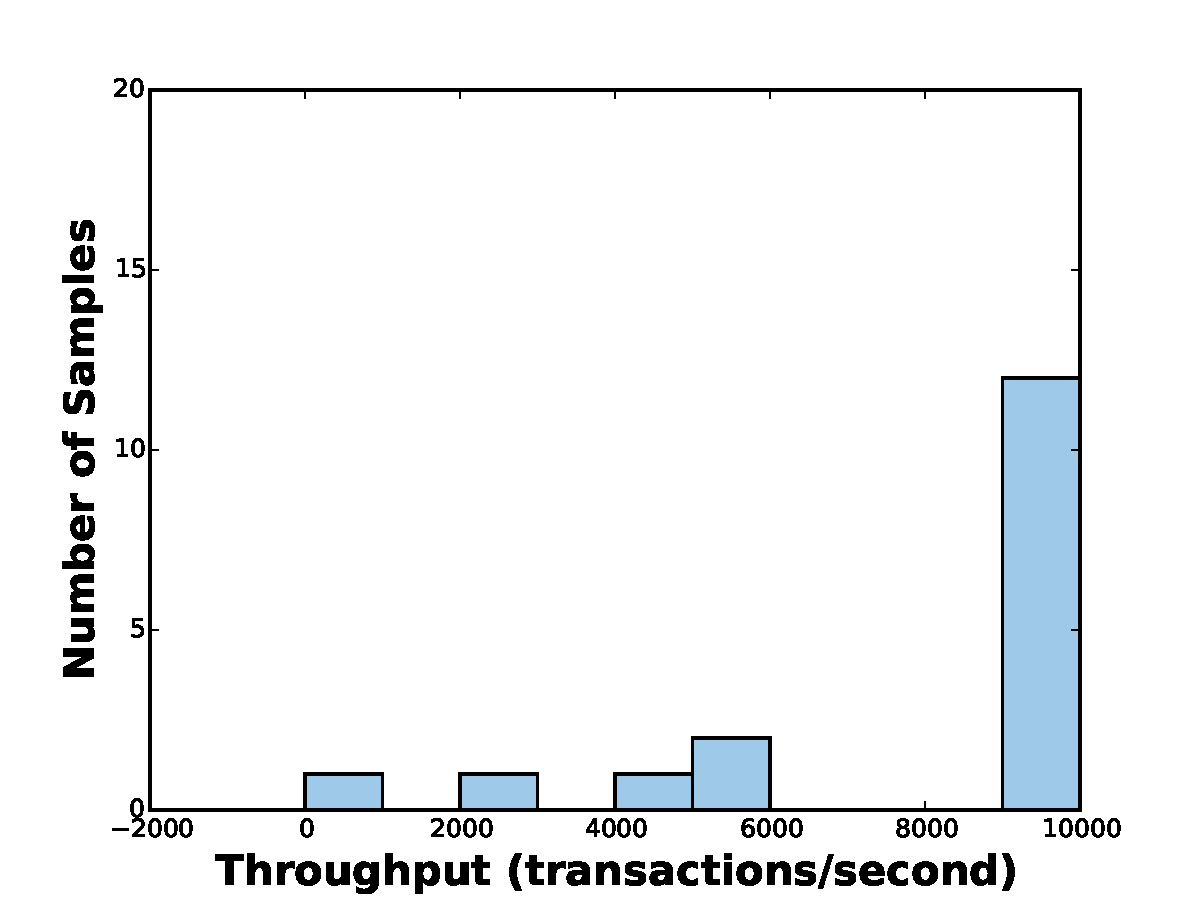
\includegraphics[width=0.4\linewidth]{figure/ycsb_balanced_test_hist_throughput_mutate.pdf}}
\subfloat[\label{fig:predicted_throughput_ycsb_balanced}]{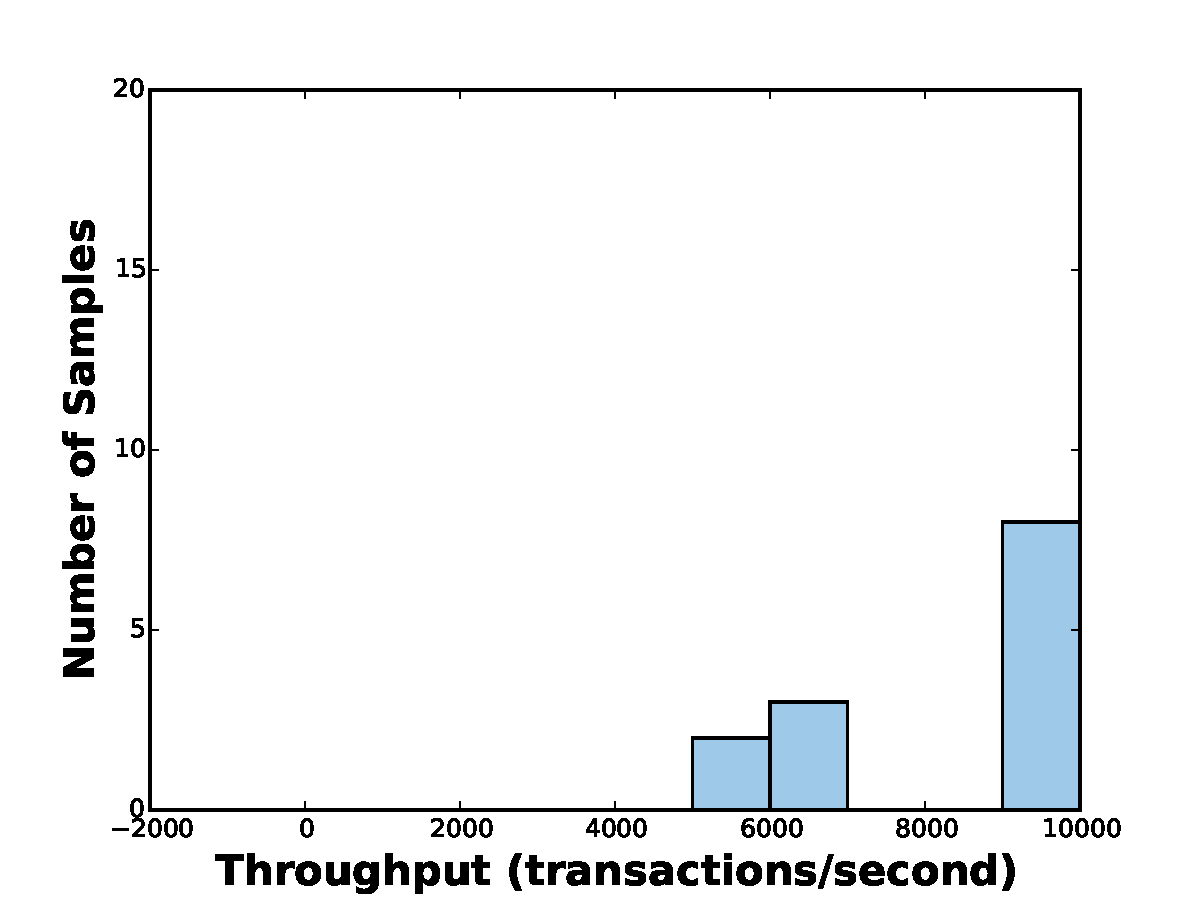
\includegraphics[width=0.4\linewidth]{figure/ycsb_balanced_pred_hist_throughput_mutate.pdf}}

\caption{(a) Actual and (b) predicted throughput distribution for the
  balanced YCSB benchmark}
\label{fig:throughput_ycsb_balanced}
\end{figure*}


The accuracy increases quickly to $91\%$ with a maximum depth of $8$. The impact
of maximum tree depth on the accuracy of the decision tree classifier
is presented in \cref{fig:tree_depth}. Using three-way cross validation,
we verified that the tree is able to classify the dataset accurately 
without overfitting. 
The impact of maximum number of leaf nodes on the accuracy of the 
decision tree classifier is presented in \cref{fig:tree_leaves}.
We observe that these parameters affect both precision and recall
equally. The accuracy increases more steeply with increasing tree
depth as expected.

\begin{table}[h!]
  \centering
  \begin{tabular}{l|llll} 
	\toprule
   		Class &  Precision  &  Recall &  F1-score  &  Support  \\    
    \midrule
		0.0   &    1.00   &   0.00   &   1.00   &     84   \\
        1.0   &    0.99   &   1.00   &   0.99   &     74   \\
        2.0   &    0.98   &   0.99   &   0.98   &     81   \\
        3.0   &    0.54   &   0.39   &   0.45   &     18   \\
        4.0   &    1.00   &   1.00   &   1.00   &     69   \\
        5.0   &    1.00   &   0.99   &   0.99   &     70   \\
        6.0   &    1.00   &   0.95   &   0.97   &     60   \\
        7.0   &    0.41   &   0.95   &   0.57   &     19   \\
        8.0   &    0.00   &   0.00   &   0.00   &     17   \\
        9.0   &    0.56   &   0.52   &   0.54   &     27   \\
    \midrule
Avg / Total   &    0.90   &   0.91   &   0.90   &    519   \\
   \bottomrule
   \end{tabular}
\caption{Per-class accuracy metrics of the decision tree with max depth = 8.}
\label{tab:dt_stats}
\end{table}



\section{Estimation} \label{sec:estimation}

\section{Conclusion} \label{sec:conclusion}

DBMS performance tuning is a niche skill that requires much experience
and experimentation to get correct. However, machine learning
techniques can help automate this process by using prior knowledge to
estimate performance without having to go through a time-consuming
experiment. To achieve this goal, we have taken a two-step approach
where we first use map a workload to a well-studied benchmark. Armed with
this information, we then use a regression estimator to estimate the
performance of the benchmark under a given environment.

Using decision trees to map the workloads, we find that we can
classify workloads using a few defining characteristics. The decision
trees produces effectively discriminate between the different
benchmarks and are very intuitive. For performance estimation, we trained estimators
using Gaussian Process Regression that show very accurate estimation
of database throughput and latency. In addition, these highly accurate
estimators can be trained with as few as 600 samples! Further analysis
of performance estimation using Lasso Regression provided key insights
into the features that are most influential in determining throughput
and latency.

While promising, this work only uses synthetic data generated from
OLTPBench. We hope to continue this work using a larger dataset that
includes mixtures of benchmarks along with real-world workloads. In
addition, we hope to extend our data to include performance
estimation across different hardware profiles and DBMS's. This larger
amount of more realistic data should help us get additional insights
about how best to estimate performance of arbitrary database workloads.

\bibliographystyle{plain}
\bibliography{ref}

\end{document}
% end doc
